\section{Taylor 展开与余项：匹配局部变化信息}
\label{sec:02-Calculus/05-Sequences-and-Series/06}

牛顿法在当前点用一个二次多项式代替目标函数，然后直接跳到这个二次模型的最小值点。跳完常常发现函数值反而变大了。模型在当前点匹配得完美无缺——函数值、梯度、二阶导都对得上——问题出在跳得太远，远到模型已经不代表原函数了。

信赖域方法的应对是给每一跳设一个半径上限，只在半径内相信模型。半径该取多大？这不是一个可以靠调参蒙混过去的问题，它问的是：一个只匹配了有限阶导数的多项式，在离中心多远的范围内还值得相信。答案藏在余项里。

\subsection{系数不需要猜}

线性化只用到函数值和一阶导数：\(P_1(x)=f(a)+f'(a)(x-a)\)。若还想让多项式在 \(a\) 处的二阶、三阶变化也与 \(f\) 一致，系数就被逐条钉死，得到

\[
P_n(x)=\sum_{k=0}^{n}\frac{f^{(k)}(a)}{k!}(x-a)^k.
\]

阶乘的来源是一句话的事：\((x-a)^k\) 求 \(k\) 次导后在 \(a\) 处取值为 \(k!\)，要让第 \(k\) 阶导数对上 \(f^{(k)}(a)\)，系数就得先把这个 \(k!\) 除掉。整个构造没有任何自由度，\(n\) 阶 Taylor 多项式由前 \(n\) 阶导数唯一确定。

到这里为止，得到的只是一个在 \(a\) 处贴得很紧的多项式。它离开 \(a\) 之后有多不靠谱，构造过程一个字也没说。

\subsection{余项才是可信度的载体}

写

\[
f(x)=P_n(x)+R_n(x),
\]

这个等式是定义，没有内容——内容全在能否给 \(R_n\) 一个界。在 \(f\) 有 \(n+1\) 阶导数的条件下，Lagrange 余项给出

\[
R_n(x)=\frac{f^{(n+1)}(\xi)}{(n+1)!}(x-a)^{n+1},\qquad \xi\ \text{介于}\ a\ \text{与}\ x\ \text{之间}.
\]

\(\xi\) 的具体位置不知道，也不需要知道。只要在关心的区间上有 \(\abs{f^{(n+1)}}\le M\)，就能收下一条可用的预算：

\[
\abs{R_n(x)}\le\frac{M}{(n+1)!}\abs{x-a}^{n+1}.
\]

右边有两个可以调的旋钮，而它们的地位完全不同。\(\abs{x-a}^{n+1}\) 随距离按 \(n+1\) 次方增长，这是信赖域半径要控制的量；\(M\) 是高阶导数的规模，由函数本身决定，你改不了它，只能去估计。开头那个跳过头的例子，就是把第一个旋钮开得太大，让 \(\abs{x-a}^{3}\) 淹没了二次模型的优势。

试一个具体的误差预算。摆的小角度线性化把 \(\sin\theta\) 换成 \(\theta\)，这一步能不能用，不该靠两条曲线看起来接近来判断。取 \(a=0\)：\(\sin\) 的二阶导数在 0 处为零，所以 \(P_2(\theta)\) 仍是 \(\theta\)，可以直接调用 \(n=2\) 的余项。三阶导数是 \(-\cos\)，绝对值不超过 1，于是 \(\abs{\sin\theta-\theta}\le\abs\theta^3/6\)，相对于线性项的误差不超过 \(\theta^2/6\)。\(\abs\theta=0.1\) 弧度时不到 \(0.17\%\)，\(\abs\theta=0.5\) 时涨到约 \(4\%\)。误差按角度的平方上升，这个界只管单次替换，不保证长时间积分出来的轨迹同样准确。

再把上一节欠下的账结掉。由 \(-\ln(1-x)=\sum x^n/n\) 换元 \(x\mapsto-x\) 得

\[
\ln(1+x)=x-\frac{x^2}2+\frac{x^3}3-\cdots,\qquad\abs x<1,
\]

而端点 \(x=1\) 不在幂级数定理的保护范围内。余项可以直接把它拿下：对 \(f(x)=\ln(1+x)\) 有 \(\abs{f^{(n+1)}(x)}=n!/(1+x)^{n+1}\le n!\) 于 \([0,1]\)，故 \(\abs{R_n(1)}\le n!/(n+1)!=1/(n+1)\to0\)。于是 \(1-\frac12+\frac13-\cdots=\ln2\)，交错级数一节预告的等式在此闭环。

\subsection{半径之外，形式仍在，意义已无}

阶数越高不一定处处更准。看 \(f(x)=\dfrac1{1+x^2}\)，它在整条实轴上光滑，没有断点也没有尖角，可它在 0 处的 Taylor 级数是

\[
1-x^2+x^4-x^6+\cdots,
\]

一个公比为 \(-x^2\) 的几何级数，收敛半径恰好是 1。

\begin{center}
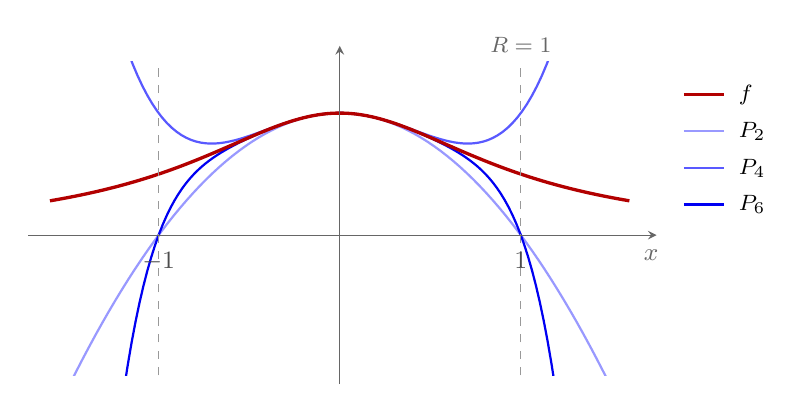
\begin{tikzpicture}[x=2.3cm,y=1.55cm,font=\small,>=stealth]
  \begin{scope}
    \clip (-1.62,-1.15) rectangle (1.62,1.42);
    \draw[blue!40,thick] plot[domain=-1.6:1.6,samples=90] (\x,{1-\x*\x});
    \draw[blue!65,thick] plot[domain=-1.6:1.6,samples=120] (\x,{1-\x*\x+\x*\x*\x*\x});
    \draw[blue!95!black,thick] plot[domain=-1.6:1.6,samples=150]
         (\x,{1-\x*\x+\x*\x*\x*\x-\x*\x*\x*\x*\x*\x});
    \draw[red!70!black,very thick] plot[domain=-1.6:1.6,samples=120] (\x,{1/(1+\x*\x)});
  \end{scope}
  \draw[black!40,dashed] (-1,-1.15) -- (-1,1.42);
  \draw[black!40,dashed] (1,-1.15) -- (1,1.42);
  \draw[->,black!60] (-1.72,0) -- (1.75,0);
  \node[below,black!60] at (1.72,-0.04) {\(x\)};
  \draw[->,black!60] (0,-1.22) -- (0,1.55);
  \node[below,black!70] at (-1,-0.06) {\(-1\)};
  \node[below,black!70] at (1,-0.06) {\(1\)};
  \node[above,black!60,font=\footnotesize] at (1,1.42) {\(R=1\)};
  \draw[red!70!black,very thick] (1.9,1.15) -- (2.12,1.15);
  \node[right,font=\footnotesize] at (2.15,1.15) {\(f\)};
  \draw[blue!40,thick] (1.9,0.85) -- (2.12,0.85);
  \node[right,font=\footnotesize] at (2.15,0.85) {\(P_2\)};
  \draw[blue!65,thick] (1.9,0.55) -- (2.12,0.55);
  \node[right,font=\footnotesize] at (2.15,0.55) {\(P_4\)};
  \draw[blue!95!black,thick] (1.9,0.25) -- (2.12,0.25);
  \node[right,font=\footnotesize] at (2.15,0.25) {\(P_6\)};
\end{tikzpicture}

\emph{虚线内侧，阶数每升高两阶，多项式就把贴合区间往外推一点。越过 \(x=\pm1\)，情况倒转：阶数越高崩得越快，\(P_6\) 比 \(P_2\) 错得更离谱。原函数在那里毫无异常，出问题的是级数。}
\end{center}

图上最反直觉的一点是右半边：在 \(\abs x>1\) 的区域，加项不是改善而是恶化。既然 \(f\) 在实轴上完全光滑，这个 \(R=1\) 是从哪里冒出来的？实轴上找不到答案。把 \(x\) 放到复平面，\(1+x^2\) 在 \(x=\pm i\) 处为零，函数在那里爆掉，而这两点到展开中心 0 的距离恰好是 1。收敛半径量的是到最近奇点的距离，而奇点可以躲在实轴之外——这也是收敛区域必须是圆盘而不是任意形状的原因。这条线索由 \hyperref[ch:069]{``复分析与留数：奇点决定函数的深层结构''} 接手。

\subsection{级数收敛，也可能收敛到别处}

半径足够大就够了吗？还不够。定义

\[
f(x)=
\begin{cases}
e^{-1/x^2},&x\ne0,\\
0,&x=0.
\end{cases}
\]

在 \(x\ne0\) 处逐次求导，得到的总是``有理式乘以 \(e^{-1/x^2}\)''的形状；\(x\to0\) 时指数因子压倒任何有理式的发散速度，极限都是 0。对这个形状作归纳可以验证 \(f\) 在 0 处无穷可微且所有阶导数为零。

于是它的 Taylor 级数恒等于 0，收敛半径是 \(\infty\)，处处收敛得漂漂亮亮。可 \(x\ne0\) 时 \(f(x)>0\)。级数收敛了，只是收敛到了另一个函数。

这个例子逼着人把三件事分开：Taylor 多项式在 \(a\) 处做有限阶的局部匹配，这总是成立；Taylor 级数作为幂级数有自己的收敛半径，这由系数决定；而级数在收敛点上是否等于 \(f\)，要靠 \(R_n(x)\to0\) 单独证明。第三件事没做，前两件做得再好也不构成函数恒等式。常见的展开——\(e^x\)、\(\sin x\)、\(\cos x\)——之所以可以放心地写成等号，是因为它们的高阶导数一致有界，余项被 \(\abs{x-a}^{n+1}/(n+1)!\) 按阶乘压到零，而不是因为它们的级数看起来收敛。

\subsection{余项界能给什么，不能给什么}

回到开头。信赖域半径的合理取值，形式上就是让 \(\dfrac{M}{(n+1)!}\abs{x-a}^{n+1}\) 小于你愿意承受的模型误差。真实算法不会去解这个不等式，因为 \(M\)——高阶导数在整个步长范围上的界——通常拿不到。实践中的做法是根据模型预测的下降量与实际下降量之比动态伸缩半径，本质上是在用观测反推那个 \(M\)。相关算法见 \hyperref[ch:076]{``优化算法：怎样把局部模型变成全局进展''}。

余项界还有两个必须记住的缺口。第一，它是关于截断的，不管浮点舍入；高阶项系数含阶乘倒数，数值上很小，与舍入误差争夺有效位，超过某个阶数之后加项只会让结果更差。第二，它是局部的：\(\abs{x-a}\) 的高次幂意味着离中心稍远误差就迅速失控，所以在 \(a\) 附近计算就应该以 \(a\) 为中心展开，Maclaurin 级数只是 \(a=0\) 的特例，没有优先地位。

一旦把眼光从一元函数移开，同一套结构会以矩阵的形式再来一次：函数值、梯度、Hessian 依次对应零阶、一阶、二阶信息，余项则决定二次模型在多大的邻域内可信。\hyperref[ch:015]{``多元微积分：变化有方向，累积有几何''} 会把这些对象一一建立起来。
